%%%% License %%%%
%Copyright (C) {2014}  {Fichou Dimitri} 
%{dimitrifichou@laposte.net}

%This program is free software; you can redistribute it and/or modify
%it under the terms of the GNU General Public License as published by
%the Free Software Foundation; either version 2 of the License, or
% any later version.

%This program is distributed in the hope that it will be useful,
%but WITHOUT ANY WARRANTY; without even the implied warranty of
%MERCHANTABILITY or FITNESS FOR A PARTICULAR PURPOSE.  See the
%GNU General Public License for more details.

%You should have received a copy of the GNU General Public License along
%with this program; if not, write to the Free Software Foundation, Inc.,
%51 Franklin Street, Fifth Floor, Boston, MA 02110-1301 USA.

%%%%%%% rTLC %%%%%%%
%%%%%%% photo.to.chrom %%%%%%%

\documentclass[a4paper]{article}\usepackage[]{graphicx}\usepackage[]{color}
%% maxwidth is the original width if it is less than linewidth
%% otherwise use linewidth (to make sure the graphics do not exceed the margin)
\makeatletter
\def\maxwidth{ %
  \ifdim\Gin@nat@width>\linewidth
    \linewidth
  \else
    \Gin@nat@width
  \fi
}
\makeatother

\definecolor{fgcolor}{rgb}{0.345, 0.345, 0.345}
\newcommand{\hlnum}[1]{\textcolor[rgb]{0.686,0.059,0.569}{#1}}%
\newcommand{\hlstr}[1]{\textcolor[rgb]{0.192,0.494,0.8}{#1}}%
\newcommand{\hlcom}[1]{\textcolor[rgb]{0.678,0.584,0.686}{\textit{#1}}}%
\newcommand{\hlopt}[1]{\textcolor[rgb]{0,0,0}{#1}}%
\newcommand{\hlstd}[1]{\textcolor[rgb]{0.345,0.345,0.345}{#1}}%
\newcommand{\hlkwa}[1]{\textcolor[rgb]{0.161,0.373,0.58}{\textbf{#1}}}%
\newcommand{\hlkwb}[1]{\textcolor[rgb]{0.69,0.353,0.396}{#1}}%
\newcommand{\hlkwc}[1]{\textcolor[rgb]{0.333,0.667,0.333}{#1}}%
\newcommand{\hlkwd}[1]{\textcolor[rgb]{0.737,0.353,0.396}{\textbf{#1}}}%

\usepackage{framed}
\makeatletter
\newenvironment{kframe}{%
 \def\at@end@of@kframe{}%
 \ifinner\ifhmode%
  \def\at@end@of@kframe{\end{minipage}}%
  \begin{minipage}{\columnwidth}%
 \fi\fi%
 \def\FrameCommand##1{\hskip\@totalleftmargin \hskip-\fboxsep
 \colorbox{shadecolor}{##1}\hskip-\fboxsep
     % There is no \\@totalrightmargin, so:
     \hskip-\linewidth \hskip-\@totalleftmargin \hskip\columnwidth}%
 \MakeFramed {\advance\hsize-\width
   \@totalleftmargin\z@ \linewidth\hsize
   \@setminipage}}%
 {\par\unskip\endMakeFramed%
 \at@end@of@kframe}
\makeatother

\definecolor{shadecolor}{rgb}{.97, .97, .97}
\definecolor{messagecolor}{rgb}{0, 0, 0}
\definecolor{warningcolor}{rgb}{1, 0, 1}
\definecolor{errorcolor}{rgb}{1, 0, 0}
\newenvironment{knitrout}{}{} % an empty environment to be redefined in TeX

\usepackage{alltt}
\usepackage{geometry}
\usepackage{eso-pic}
\usepackage{graphicx} 
\usepackage{longtable}
\usepackage[utf8]{inputenc}
\geometry{verbose,tmargin=2cm,bmargin=2cm,lmargin=2cm,rmargin=2cm}
\IfFileExists{upquote.sty}{\usepackage{upquote}}{}
\begin{document}
%%%%%%






% latex table generated in R 3.2.0 by xtable 1.8-0 package
% Thu Nov 12 12:05:20 2015
\begin{table}[ht]
\centering
\begin{tabular}{ll}
  \hline
  \hline
batch file & rTLC\_demobatch.xls \\ 
  picture file 1 & rTLC\_demopicture.JPG \\ 
   \hline
\end{tabular}
\end{table}

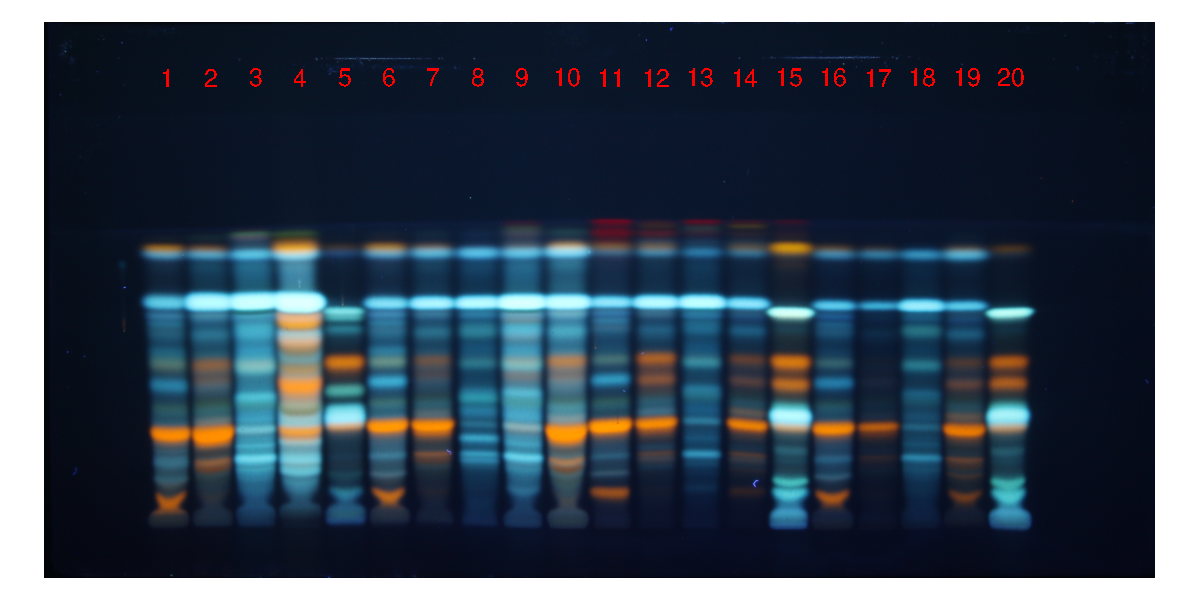
\includegraphics[width=\maxwidth]{figure/unnamed-chunk-1-1} 


% latex table generated in R 3.2.0 by xtable 1.8-0 package
% Thu Nov 12 12:05:21 2015
\begin{longtable}{rlll}
  \hline
id & Reference & Drug & Information \\ 
  \hline
  1 & T411 & Mentha & Dry Extract EtOH60 \\ 
    2 & B247 & Sage & Dry Extract EtOH60 \\ 
    3 & H329 & Melissa & Dry Extract EtOH60 \\ 
    4 & C244 & Rosmarin & Dry Extract EtOH60 \\ 
    5 & R411 & Artichoke & Dry Extract EtOH60 \\ 
    6 & N712 & Mentha & Dry Extract EtOH60 \\ 
    7 & X147 & Sage & Dry Extract EtOH60 \\ 
    8 & T105 & Melissa & Dry Extract EtOH60 \\ 
    9 & F305 & Melissa & Dry Extract EtOH60 \\ 
   10 & P236 & Sage & Dry Extract EtOH60 \\ 
   11 & A708 & Mentha & drug EtOH60 \\ 
   12 & W313 & Sage & drug EtOH60 \\ 
   13 & W247 & Melissa & drug EtOH60 \\ 
   14 & E410 & Sage & drug EtOH60 \\ 
   15 & E408 & Artichoke & drug EtOH60 \\ 
   16 & A708 & Mentha & drug H2O \\ 
   17 & W313 & Sage & drug H2O \\ 
   18 & W247 & Melissa & drug H2O \\ 
   19 & E410 & Sage & drug H2O \\ 
   20 & E408 & Artichoke & drug H2O \\ 
   \hline
\hline
\end{longtable}



\begin{knitrout}
\definecolor{shadecolor}{rgb}{0.969, 0.969, 0.969}\color{fgcolor}
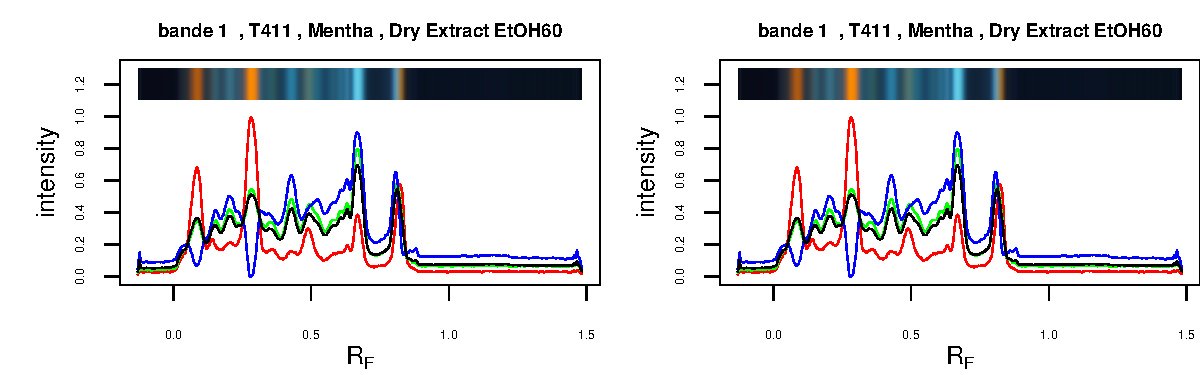
\includegraphics[width=\maxwidth]{figure/unnamed-chunk-3-1} 

\end{knitrout}

% latex table generated in R 3.2.0 by xtable 1.8-0 package
% Thu Nov 12 12:05:21 2015
\begin{table}[ht]
\centering
\begin{tabular}{ll}
  \hline
name & value \\ 
  \hline
Standard.Normal.Variate & TRUE \\ 
  Mean.centering & TRUE \\ 
   \hline
\end{tabular}
\end{table}



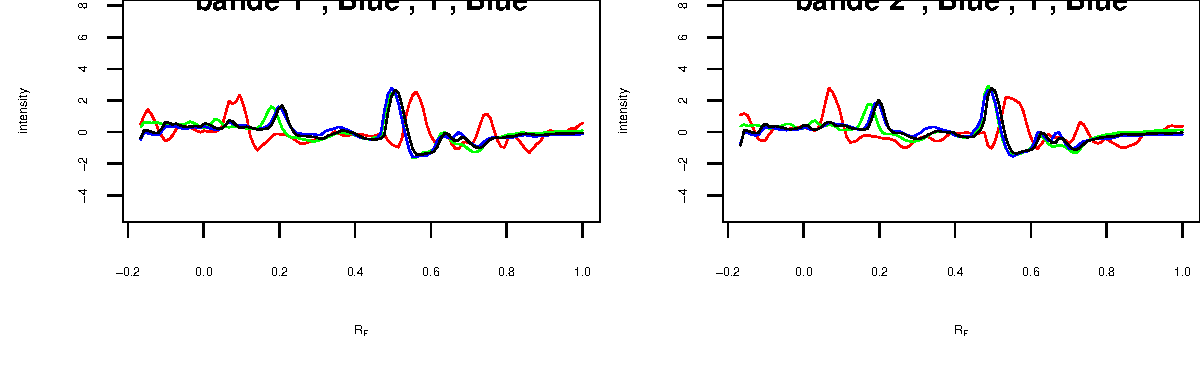
\includegraphics[width=\maxwidth]{figure/unnamed-chunk-5-1} 





% latex table generated in R 3.2.0 by xtable 1.8-0 package
% Thu Nov 12 12:05:21 2015
\begin{table}[ht]
\centering
\begin{tabular}{llrr}
  \hline
use & channel & start & stop \\ 
  \hline
FALSE & 1 & -0.13 & 1.48 \\ 
  TRUE & 2 & 0.57 & 1.48 \\ 
  TRUE & 3 & -0.13 & 1.48 \\ 
  TRUE & 4 & -0.13 & 1.48 \\ 
  FALSE & 1 & -0.13 & 1.48 \\ 
  FALSE & 2 & -0.13 & 1.48 \\ 
  FALSE & 3 & -0.13 & 1.48 \\ 
  FALSE & 4 & -0.13 & 1.48 \\ 
  FALSE & 1 & -0.13 & 1.48 \\ 
  FALSE & 2 & -0.13 & 1.48 \\ 
  FALSE & 3 & -0.13 & 1.48 \\ 
  FALSE & 4 & -0.13 & 1.48 \\ 
   \hline
\end{tabular}
\end{table}




\end{document}
